\documentclass[10pt]{article}
\usepackage{amsmath}
\usepackage{listings}
\usepackage{graphicx}
\graphicspath{ {./images/} }
\begin{document}
{\centering
    CSU44061 Machine Learning - Week 2
    \par
    Samuel Petit - 17333946
    \par
    Dataset \# id:9--9--9 
    \par
}
\section*{Question a}
Code for all questions provided in the appendix.

\subsection*{Part i}

Using matplotlib with python to generate graphs, I plotted X2 against X1 (both features)
and made the colour of the marker different based on the prediction.
The red colour represents a positive prediction (+1) and the blue colour represents a negative
prediction (-1)

\vspace{5mm} %5mm vertical space

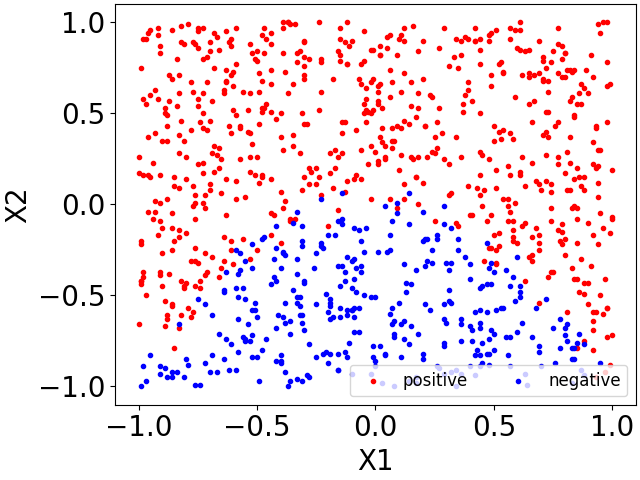
\includegraphics[scale=0.35]{Figure_1.png}

\subsection*{Part ii}
Using code provided in the appendix, I trained a logistic regression
classifier which gave me the following model:

\begin{equation*}
    \theta_{0} + \theta_{1}x_{1} + \theta_{2}x_{2} = -1.91100581 - 0.18987022 * x_{1} - 5.76650534 * x_{2}
\end{equation*}

\subsection*{Part iii}
The following plot plots X1 against X2, using the predictions and
the actual y output from the dataset.
The y output and predictions use different colours and markers to attempt to marke
this graph more readible.



It is a bit hard to see however we can clearly see that the predictions
are quite rough and very inacurrate on the edges as well as the top of the
slope.

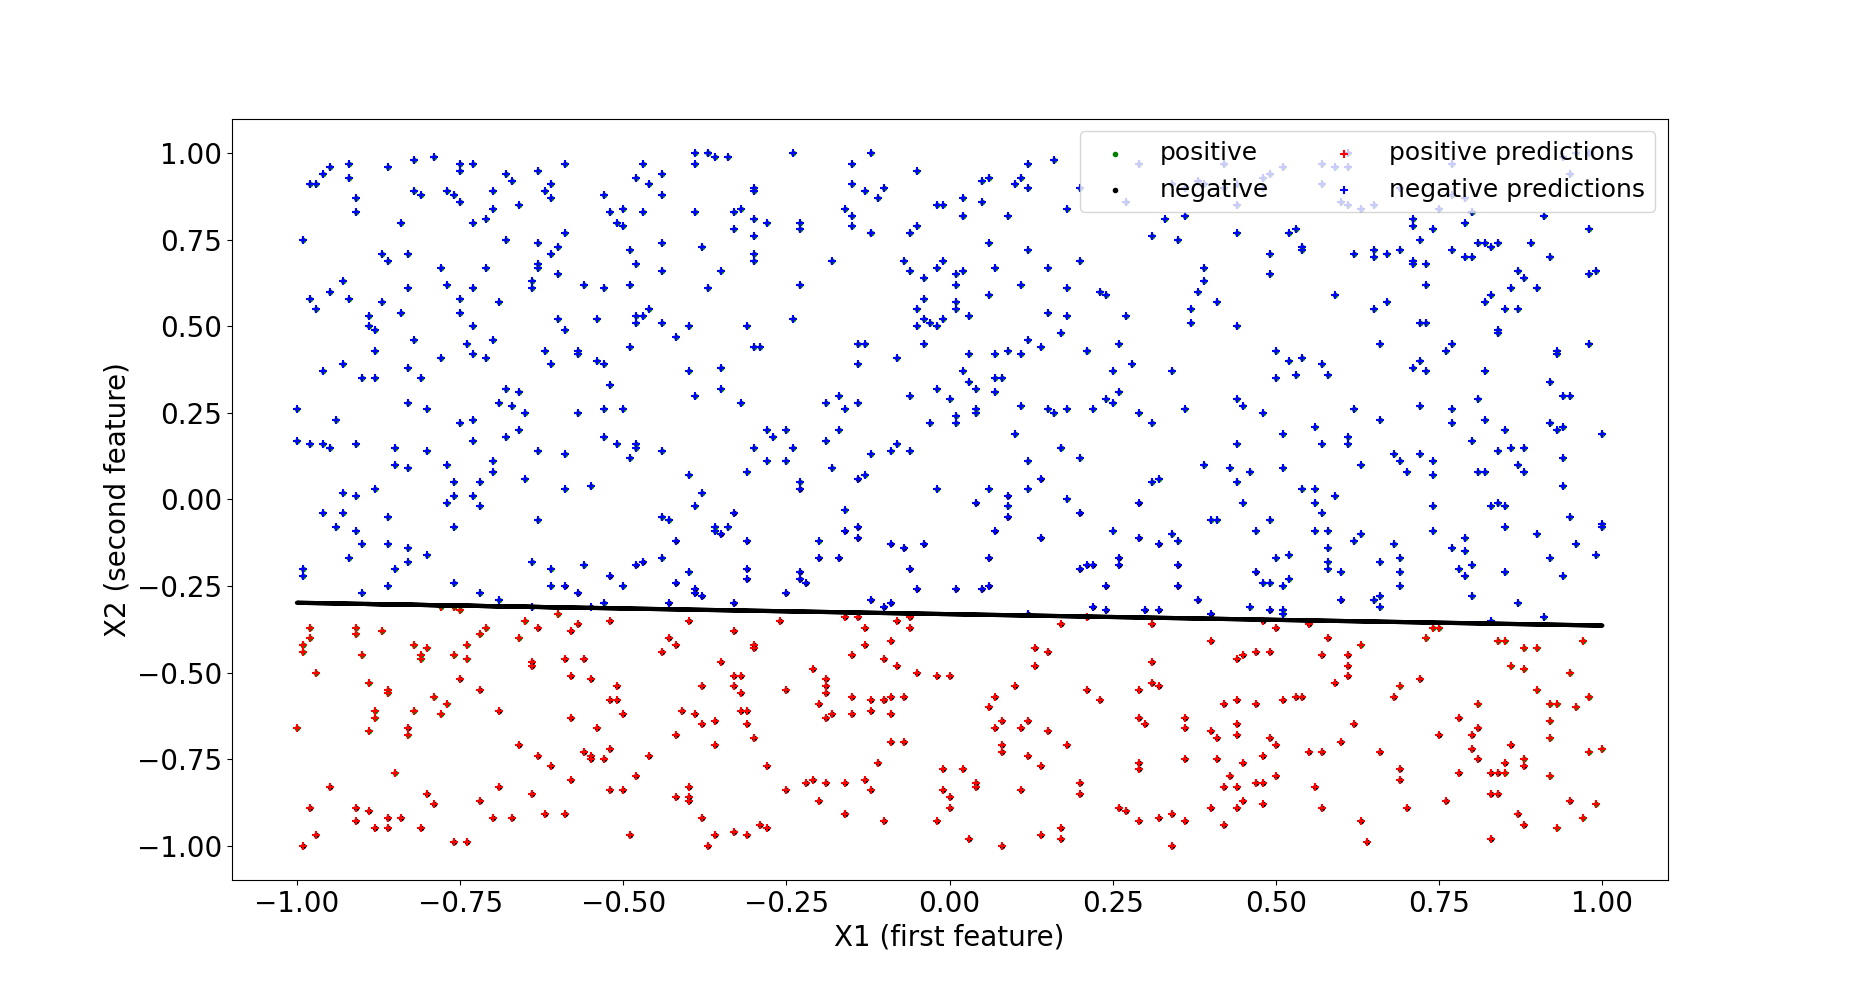
\includegraphics[scale=0.245]{Figure_2.png}

As for the slope representing the classifier separation, I used the
following equation. It is obtained by computing the sum of the linear function
which uses $\theta_{0}$ and $\theta_{1}$ and dividing the result
by the 3rd value of the model: $\theta_{2}$.

\begin{equation*}
    y = -\frac{\theta_{1} * x_{1}^{i} + \theta_{0}}{\theta_{2}}
\end{equation*}

\section*{Question b}
\subsection*{Part i}
Using code provided in the appendix, I trained a linear SVM
classifier with 3 different C values. I obtained the following parameters:

C = 0.001
\begin{equation*}
    -0.21517665 - 0.00849777 * x_{1} - 0.47908454 * x_{2}
\end{equation*}

C = 1
\begin{equation*}
    -0.61452025 - 0.06661916 * x_{1} - 1.88463746 * x_{2}
\end{equation*}

C = 1000
\begin{equation*}
    -0.62224281 - 0.06807451 * x_{1} - 1.90613439 * x_{2}
\end{equation*}



It is worth noting that using C = 1000 required a maximum amount of iterations
when training the model to be much higher. I used a maximum of 100000 iterations
for this algorithm.

\subsection*{Part ii}
Using the same method for plotting as in the previous question,
I plot the predictions on top of the actual values in order to try
detect inconsistencies on the predictions. The separation
line is also plotted using the same function as explained
in the previous question. Using the different values for C we
obtain the following graphs:

C = 0.001

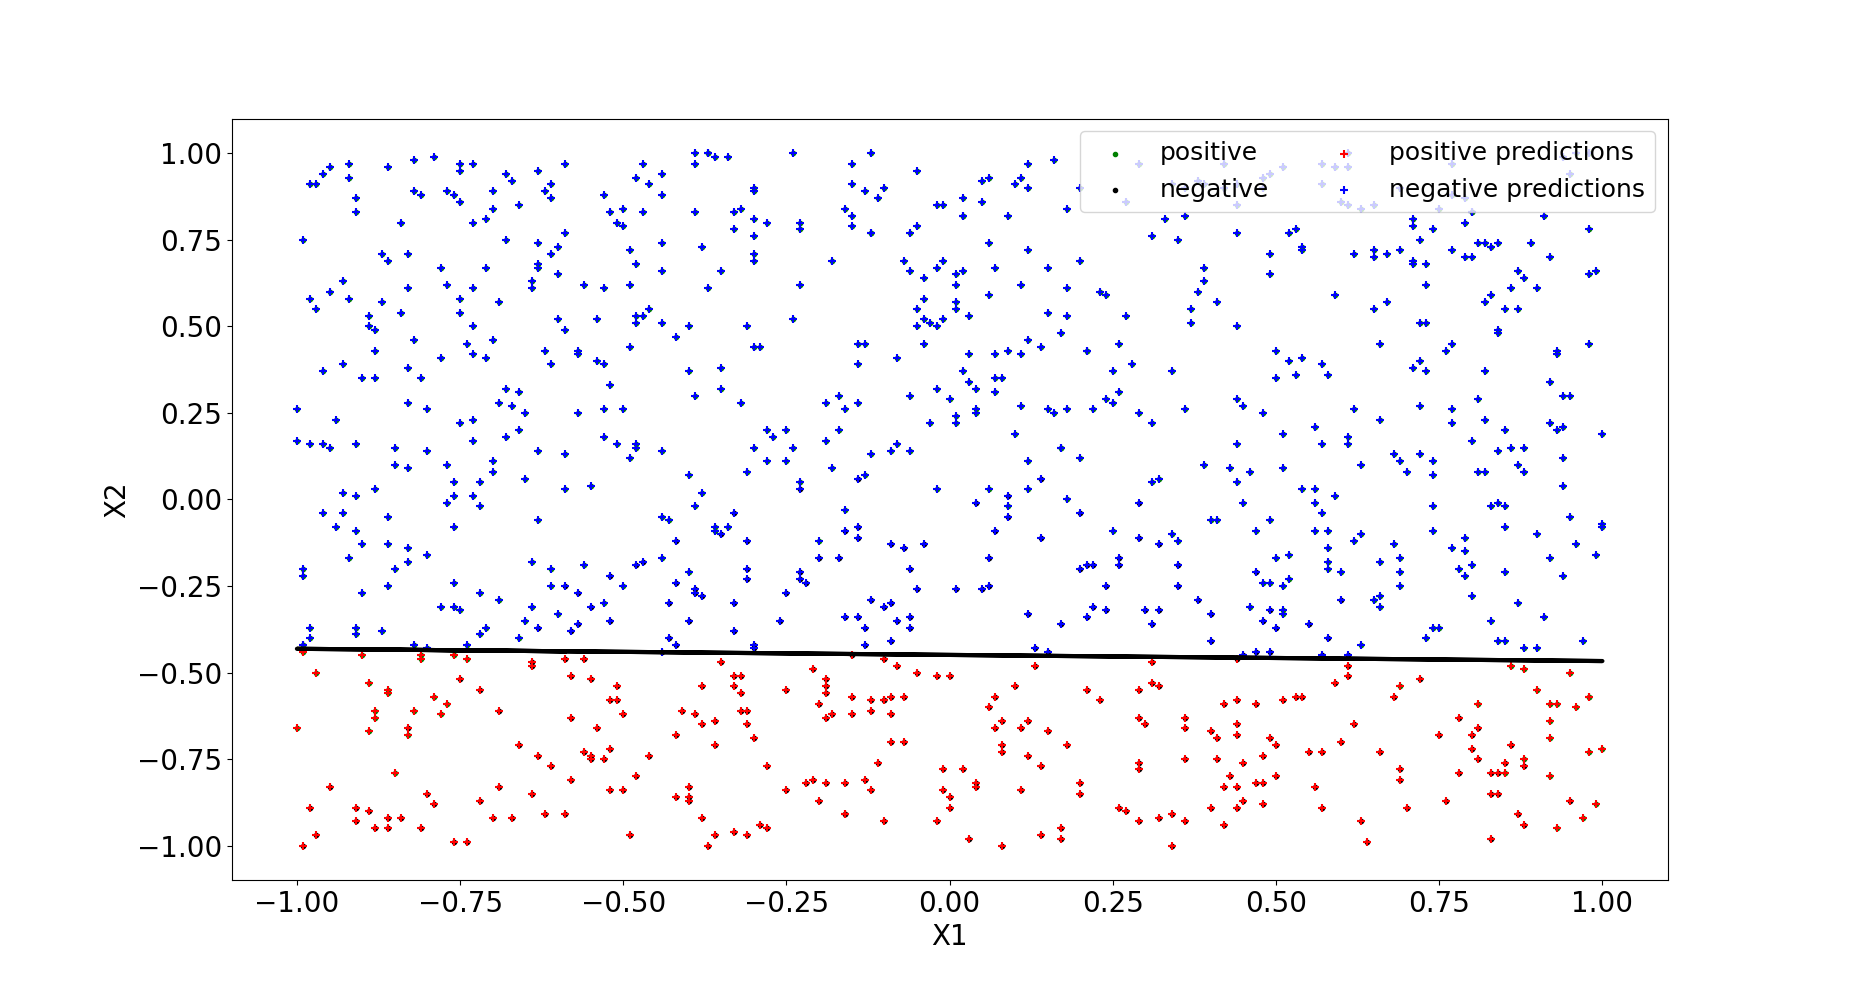
\includegraphics[scale=0.245]{Figure_C_0001.png}

C = 1

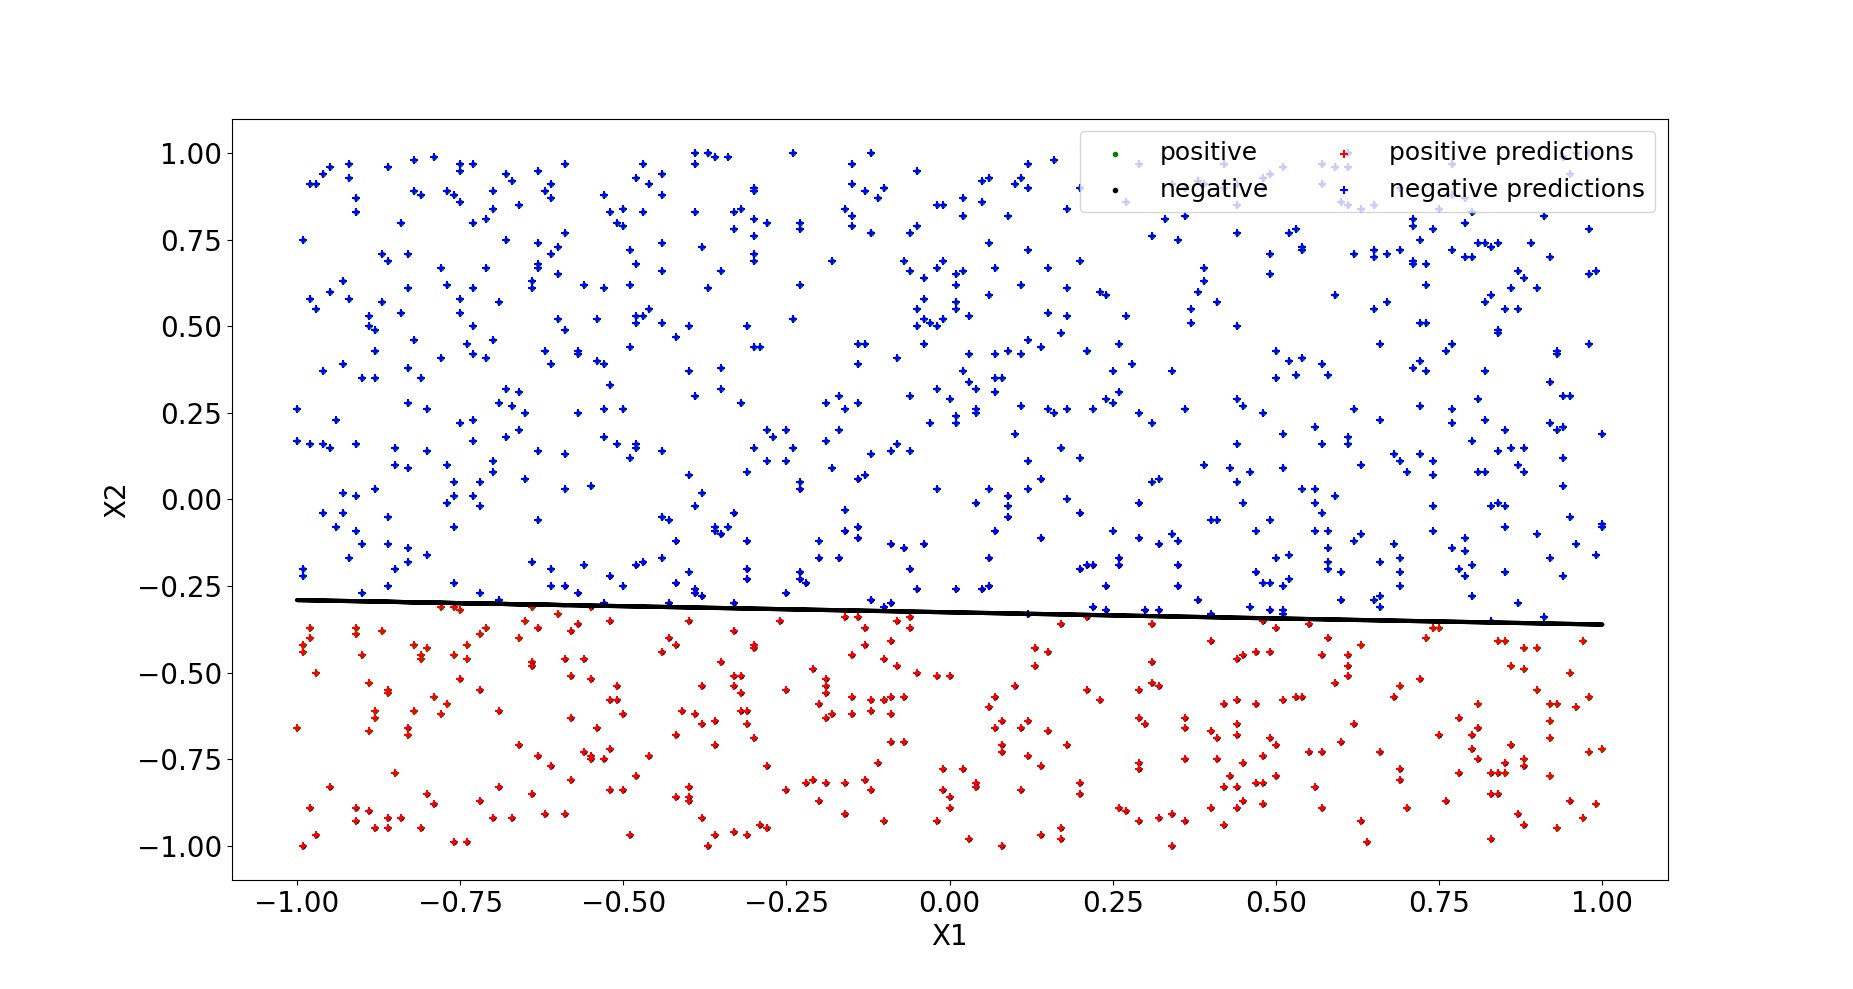
\includegraphics[scale=0.245]{Figure_C_1.png}


C = 1000

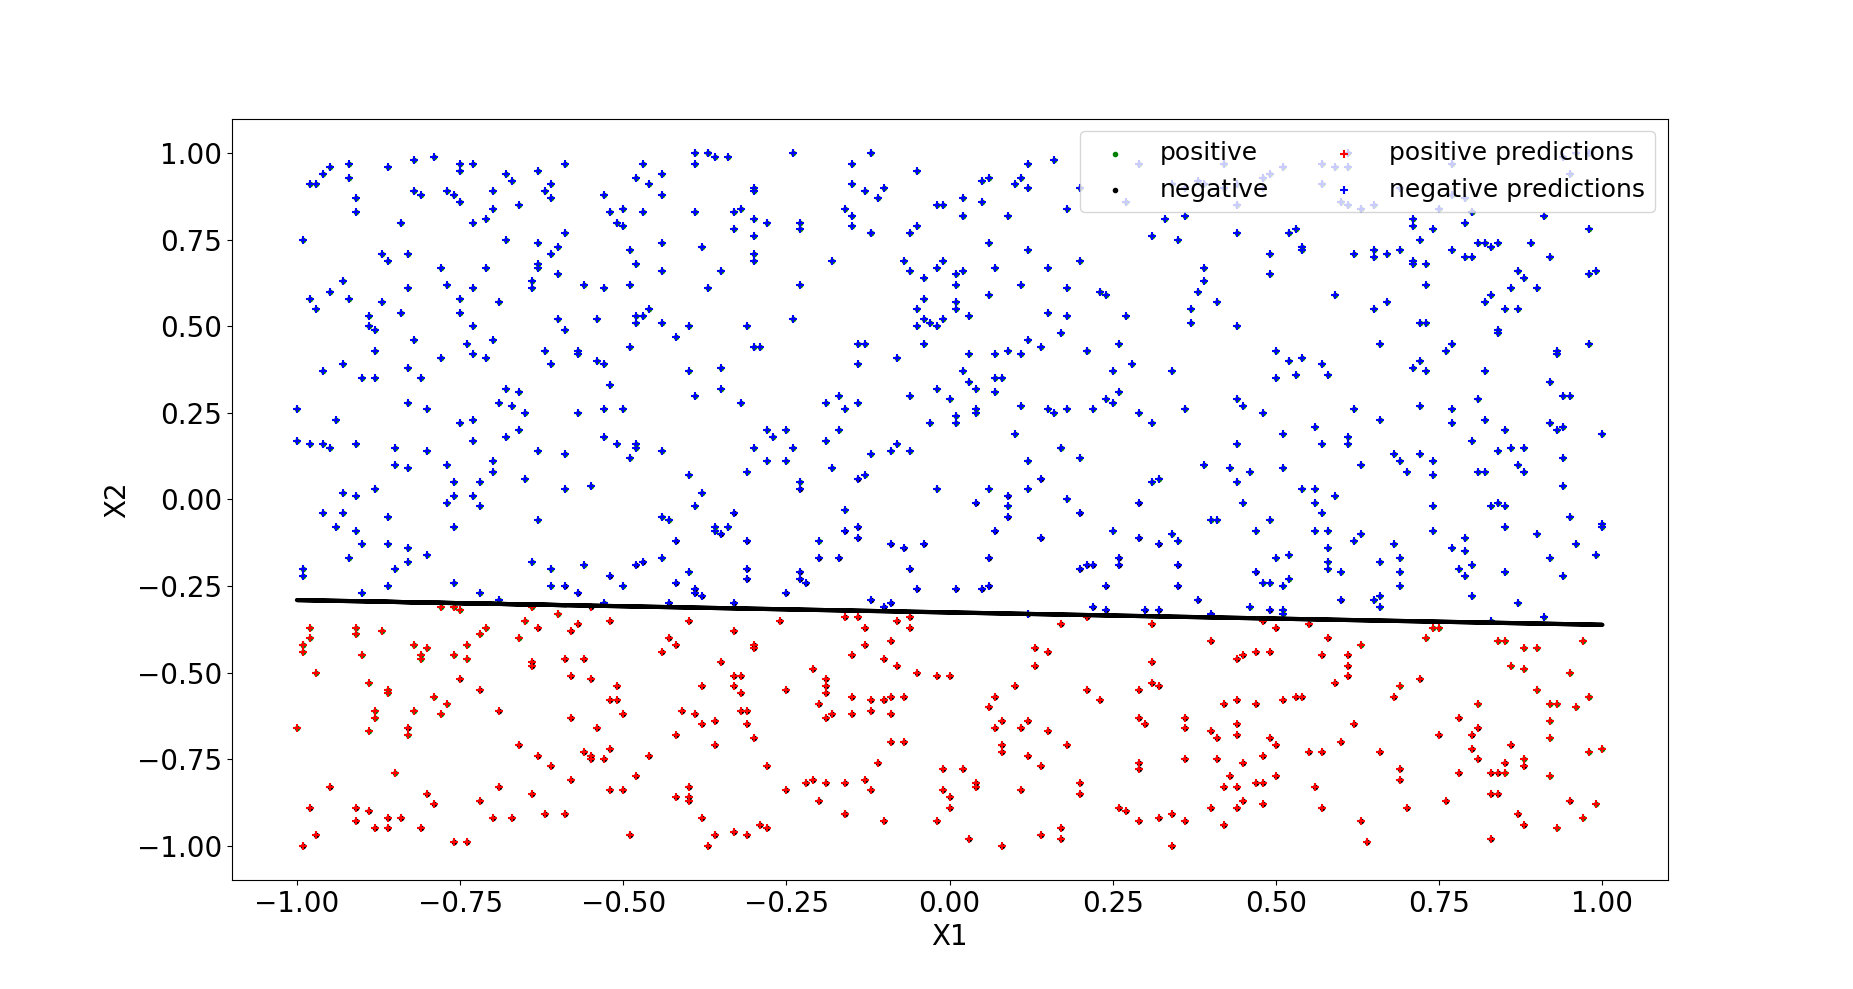
\includegraphics[scale=0.245]{Figure_C_1000.png}

\subsection*{Part iii}
A larger value for C will choose a smaller margin for the hyperplane
separating our data. In this case this results in a higher intercept value
and smaller coefficient. A smaller value for C will make the margin for data separation
bigger, potentially resulting in more misclassifications.

Looking at the plot, a higher value for C makes the separating line for the predictions
higher on the y axis (representing X2), thus prediciting more values as positive (y = 1).

A lower value for C makes the separating line lower on the y axis, thus predicting less values
as positive (y = 1).

In our situation it seems that a larger value for C works best.

\section*{Question c}
\subsection*{Part i}
I created two additional features by squaring both features
$X1$ and $X2$. This gives me a total of 4 features to use to train 
a logistic regression classifier. Using code provided in the appendix
we get the following parameters:

\begin{equation*}
    \theta_{0} + \theta_{1}x_{1} + \theta_{2}x_{2} +  \theta_{3}x_{1}^{2} + \theta_{4}x_{2}^2 
\end{equation*}
\begin{equation*}
    = 0.34532747- 0.61211948 * x_{1} - 20.55468232 * x_{2} - 22.19408429 * x_{1}^{2} + 2.27234931 * x_{2}^{2} 
\end{equation*}

\subsection*{Part ii}
Using the same system as with previous graphs, I plotted
the predictions on top of the actual outputs values. This
plot is X1 against X2, where actual outputs and predictions are
plotted with different colours and markers using a model with 4 features
as described in the previous section.


We notice that predictions are much better than our previous models.

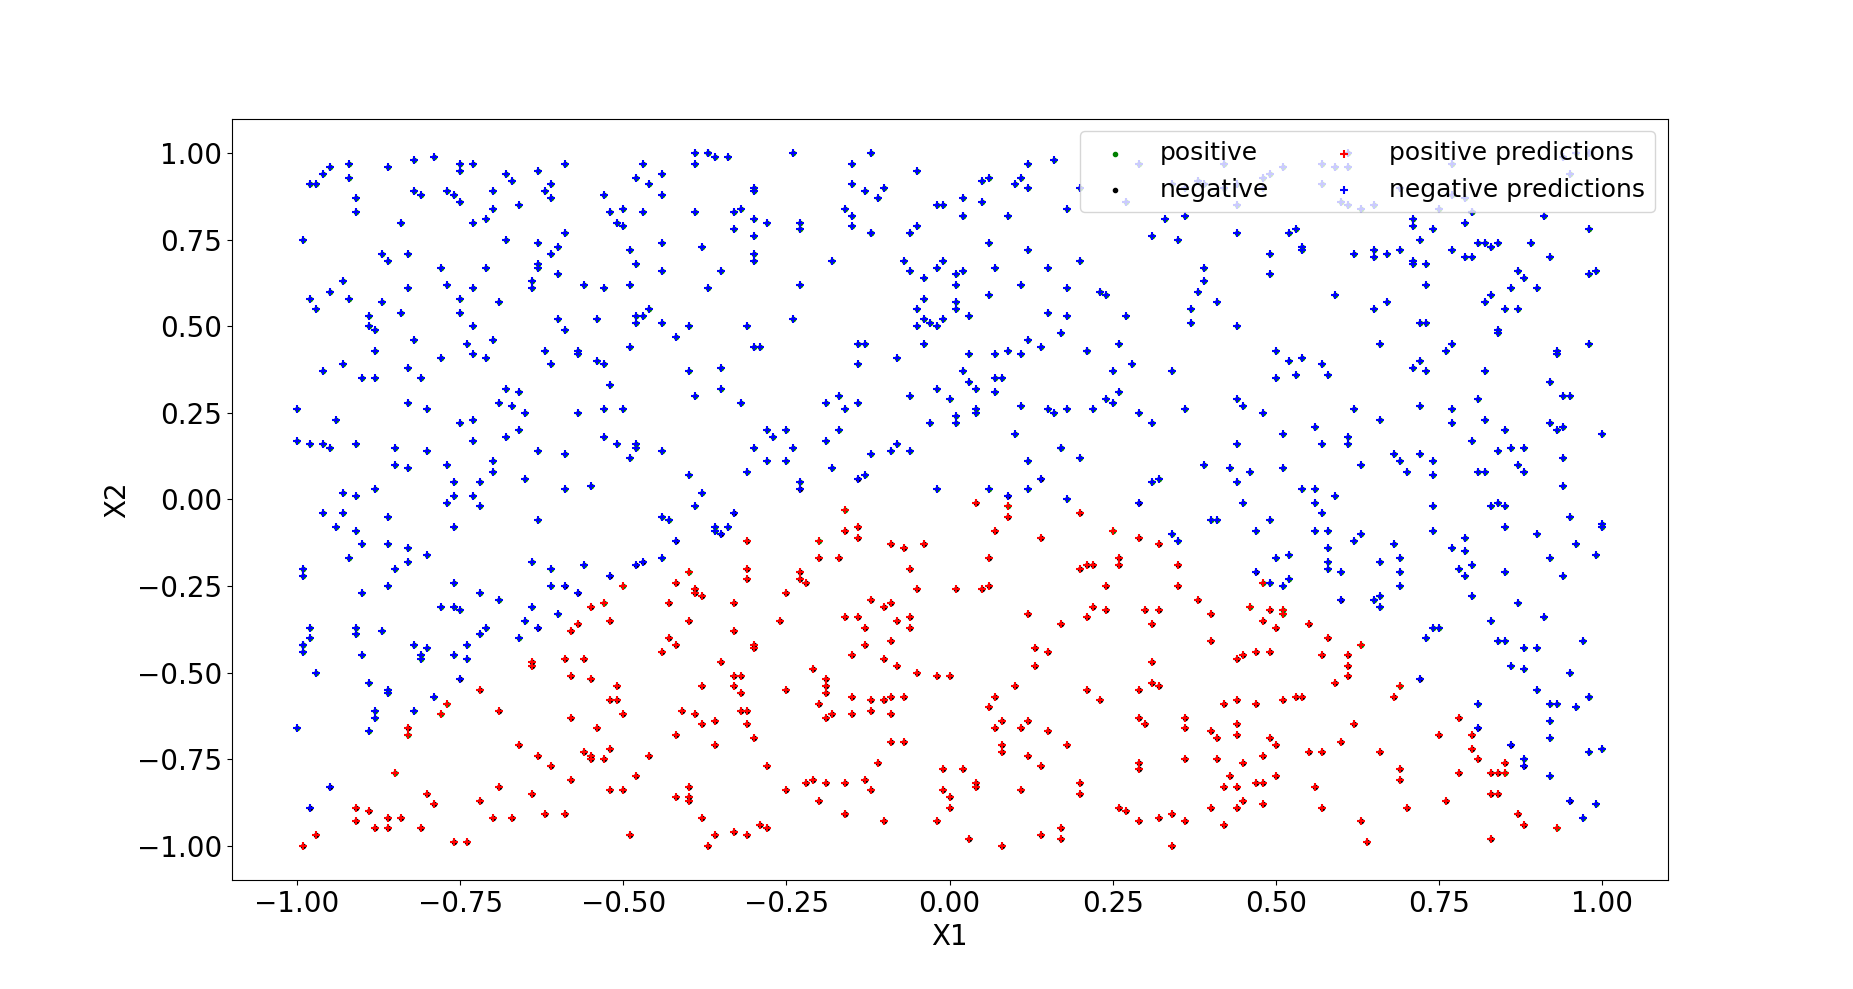
\includegraphics[scale=0.245]{Figure_3.png}

\section*{Appendix}
Util methods:
\begin{lstlisting}[language=Python]
import numpy as np
import pandas as pd

def get_data():
    # Read in data
    df = pd.read_csv("week2.csv", comment='#')
    X1 = df.iloc[:, 0]
    X2 = df.iloc[:, 1]
    X = np.column_stack((X1, X2))
    y = df.iloc[:, 2]
    ytrain = np.sign(y)
    return X1, X2, X, y, ytrain

\end{lstlisting}
Question A i:
\begin{lstlisting}[language=Python]
import matplotlib.pyplot as plt
from util import get_data

# Read in data
X1, X2, X, y, ytrain = get_data()

# Plot the data
plt.rc('font', size=20)
plt.rcParams['figure.constrained_layout.use'] = True
neg = plt.scatter(X1[y < 0], X2[y < 0],
                color='red', marker=".")
pos = plt.scatter(X1[y > 0], X2[y > 0],
                color='blue', marker=".")
plt.xlabel("X1")
plt.ylabel("X2")
plt.legend((neg, pos), ["positive", "negative"],
            scatterpoints=1,
            loc='lower right',
            ncol=2,
            fontsize=12)
plt.show()
\end{lstlisting}
Question A ii and iii:
\begin{lstlisting}[language=Python]
from sklearn.linear_model import LogisticRegression
import matplotlib.pyplot as plt
from util import get_data
import numpy as np

# Read in data
X1, X2, X, y, ytrain = get_data()

# Train the model
model = LogisticRegression(solver='lbfgs', 
                            penalty="none")
model.fit(X, ytrain)

# Print model values
print("Logistic Regression Classifier")
print("intercept:", model.intercept_)
print("slope:", model.coef_)

# Predict values
ypred = np.sign(model.predict(X))

# Extract the slope to display from model coefs
line_bias = model.intercept_
line_w = model.coef_.T
points_y = [(line_w[0]*x+line_bias)/(-1*line_w[1])
                                    for x in X1]

# Plot the preditions
plt.rc('font', size=20)
pos = plt.scatter(X1[y > 0], X2[y > 0],
                    color='black', marker=".")
neg = plt.scatter(X1[y < 0], X2[y < 0],
                    color='green', marker=".")
pos_pred = plt.scatter(X1[ypred > 0], X2[ypred > 0],
                        color='red', marker="+")
neg_pred = plt.scatter(X1[ypred < 0], X2[ypred < 0],
                        color='blue', marker="+")
plt.rcParams['figure.constrained_layout.use'] = True
plt.xlabel("X1 (first feature)")
plt.ylabel("X2 (second feature)")
plt.plot(X1, points_y, color='black', linewidth=3)
plt.legend((neg, pos, pos_pred, neg_pred), 
            ["positive", "negative",
            "positive predictions",
            "negative predictions"],
            scatterpoints=1,
            loc='upper right',
            ncol=2,
            fontsize=18)
plt.show()
    
\end{lstlisting}
Question b
\begin{lstlisting}[language=Python]
from sklearn.svm import LinearSVC
import matplotlib.pyplot as plt
from util import get_data
import numpy as np

# Read in data
X1, X2, X, y, ytrain = get_data()

# Train Linear SVC for C=0.001, 1 and 1000
for C_val in [0.001, 1, 1000]:
    # max iter lower than 100 000 
    #makes C=1000 not converge
    model = LinearSVC(C=C_val, max_iter=100000)
                    .fit(X, ytrain)
    print("C, intercept, slope",
        C_val, model.intercept_, model.coef_)

# Plot one of the 3 models 
# (change C value to plot the other ones)
model = LinearSVC(C=0.001, max_iter=100000)
                .fit(X, ytrain)
line_bias = model.intercept_
line_w = model.coef_.T
points_y = [(line_w[0]*x+line_bias)
            / (-1*line_w[1]) for x in X1]

# Predict values
ypred = np.sign(model.predict(X))

# Plot the preditions
plt.rc('font', size=20)
pos = plt.scatter(X1[y > 0], X2[y > 0],
                    color='black', marker=".")
neg = plt.scatter(X1[y < 0], X2[y < 0],
                    color='green', marker=".")
pos_pred = plt.scatter(X1[ypred > 0], X2[ypred > 0],
                        color='red', marker="+")
neg_pred = plt.scatter(X1[ypred < 0], X2[ypred < 0],
                        color='blue', marker="+")
plt.rcParams['figure.constrained_layout.use'] = True
plt.xlabel("X1")
plt.ylabel("X2")
plt.plot(X1, points_y, color='black', linewidth=3)
plt.legend((neg, pos, pos_pred, neg_pred),
            ["positive", "negative",
            "positive predictions",
            "negative predictions"],
            scatterpoints=1,
            loc='upper right',
            ncol=2,
            fontsize=18)
plt.show()
\end{lstlisting}
Question c
\begin{lstlisting}
import matplotlib.pyplot as plt
from sklearn.linear_model import LogisticRegression
import matplotlib.pyplot as plt
from util import get_data
import numpy as np
import pandas as pd
from sklearn.preprocessing import PolynomialFeatures

# Read in data
X1, X2, X, y, ytrain = get_data()

X1 = np.array(X1)
X2 = np.array(X2)
# Square both features
X1_square = X1.reshape(-1, 1)
X2_square = X2.reshape(-1, 1)
X1_square = np.square(X1)
X2_square = np.square(X2)
X = np.column_stack((X1, X2, X1_square, X2_square))

# Train our model
model = LogisticRegression(solver='lbfgs',
                            penalty="none")
model.fit(X, ytrain)

# Print model values
print("Logistic Regression Classifier")
print("intercept:", model.intercept_)
print("slope:", model.coef_)

# Predict values
ypred = np.sign(model.predict(X))

# Plot the preditions
plt.rc('font', size=20)
pos = plt.scatter(X1[y > 0], X2[y > 0],
                    color='black', marker=".")
neg = plt.scatter(X1[y < 0], X2[y < 0],
                    color='green', marker=".")
pos_pred = plt.scatter(X1[ypred > 0], X2[ypred > 0],
                        color='red', marker="+")
neg_pred = plt.scatter(X1[ypred < 0], X2[ypred < 0],
                        color='blue', marker="+")
plt.rcParams['figure.constrained_layout.use'] = True
plt.xlabel("X1")
plt.ylabel("X2")
plt.legend((neg, pos, pos_pred, neg_pred), 
            ["positive", "negative", 
            "positive predictions",
            "negative predictions"],
            scatterpoints=1,
            loc='upper right',
            ncol=2,
            fontsize=18)
plt.show() 
\end{lstlisting}
\end{document}
